\documentclass[dvisvgm, tikz, border=4pt]{standalone}
\begin{document}
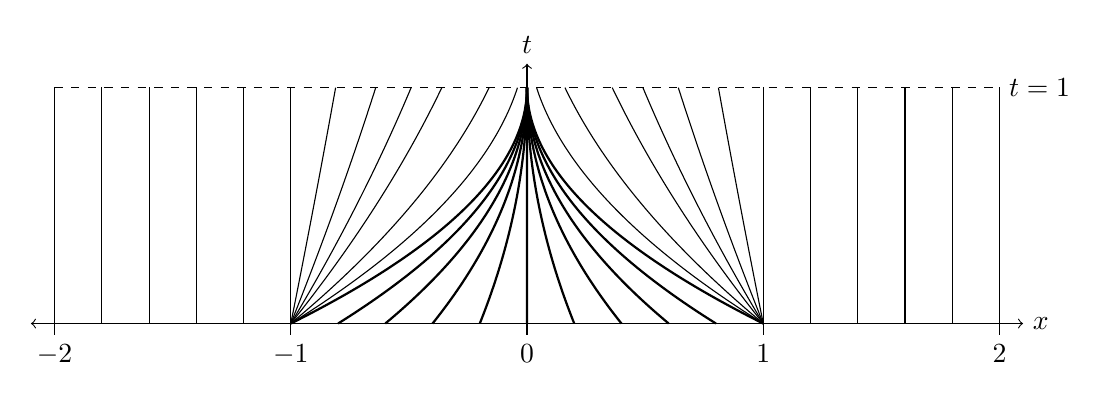
\begin{tikzpicture}[scale=3]
  % axes
  \draw[<->] (-2.1,0) -- (2.1,0) node[right] {$x$};
  \draw[->] (0,0) -- (0,1.1) node[above] {$t$};
  \foreach \x in {-2,-1,0,1,2}
    \draw (\x,0.05) -- (\x,-0.05) node[below] {$\x$};

  % the line t = 1
  \draw[dashed] (-2,1) -- (2,1) node[right] {$t=1$};

  % |x| > 1: u = 0, characteristics are vertical
  \foreach \a in {-2,-1.8,-1.6,-1.4,-1.2,-1,1,1.2,1.4,1.6,1.8,2}
    \draw (\a,0) -- (\a,1);

  % |x| < 1: u = -1, characteristics x = a(1-t)^2 focus at the origin
  \foreach \a in {-1,-0.8,...,1}
    \draw[thick] plot[domain=0:1, samples=100, variable=\t] ({\a*(1-\t)^2}, \t);

  % rarefaction fans from x = 1 and x = -1
  \foreach \c in {0.1,0.2,0.3,0.4,0.6,0.8} {
    \draw[thin] plot[domain=0:1, samples=100, variable=\t] ({ (1-\c*\t)^2}, \t);
    \draw[thin] plot[domain=0:1, samples=100, variable=\t] ({-(1-\c*\t)^2}, \t);
  }
\end{tikzpicture}
\end{document}
